\documentclass[fleqn]{article}
\usepackage[utf8]{inputenc}
\usepackage{polski}
\usepackage{amsmath, bm}
\usepackage{titlesec}
\usepackage{graphicx}
\usepackage{caption}
\usepackage{subcaption}
\usepackage[margin= 2.8cm]{geometry}

\title{Metody interpolacji}
\author{Piotr Pesta, 184531}
\date{Maj 2022}
\setlength{\parindent}{20pt}

\graphicspath{{./Plots/}}


\begin{document}
\titlelabel{\thetitle.\quad}
\maketitle


\section{Wstęp}
    Celem projektu było zaimplementowanie dwóch metod interpolacji: metody Lagrange'a oraz funkcji skelejancyh.
    W reazlizacji zadania skorzystałem z biblioteki matplotlib do rysowania wykresów oraz modułu os do pobierania informacji o plikach w folderze.

\section{Ogólne założenia}
    Liczba n oznaczać będzie liczbę węzłów interpolacji, a więc przedziałów interpolacji będzie n-1.
\newpage
\section{Metoda Lagrange'a}
    Metoda Lagrange'a korzysta z faktu, że n+1 punktów definiuje jednoznacznie wielomian n-tego stopnia. 
    Wartość funkcji interpolującej w dowolnym punkcie x wynosi:

    
    \[ 
        F(x) = \sum_{i = 0}^{n} y_i\phi_i(x)   
   \]
   \[
        \phi_i(x) = \prod_{j=0, j \neq i}^n \frac{x - x_j}{x_i - x_j}     
   \]

    \noindent Zaletą tej metody jest fakt, że nie trzeba tworzyć i rozwiązywać układu równań, co może być kosztowne obliczeniowo.
    Największą jej wadą jest natomiast efekt Rungego, który pojawia się przy interpolacji równo-odległych punktów przy użyciu wielomianów
    wysokiego stopnia. Efekt Rungego polega na pojawianiu się oscylacji na krańcach przedziału interpolacji. Zaczyna być widoczny dla n = 10,
    a wraz ze wzrostem n, oscylacje stają się coraz większe.

    \begin{figure}[h]
        \centering
        \begin{subfigure}{.5\textwidth}
          \centering
          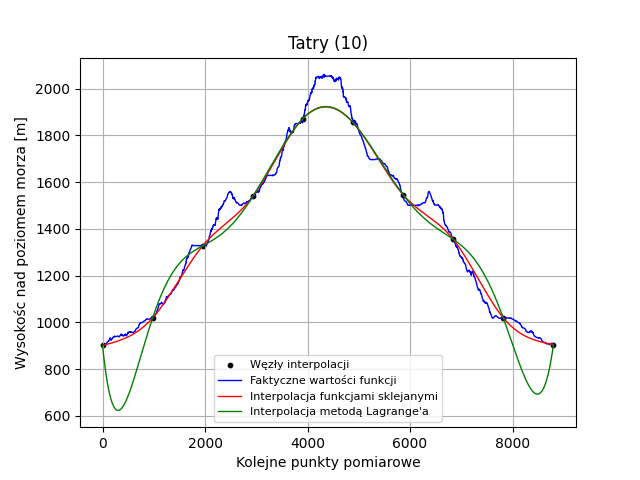
\includegraphics[width=\linewidth]{plot_10_points_Tatry.png}
          \caption{Przykład dla n = 10}
          \label{fig:sub1}
        \end{subfigure}%
        \begin{subfigure}{.5\textwidth}
          \centering
          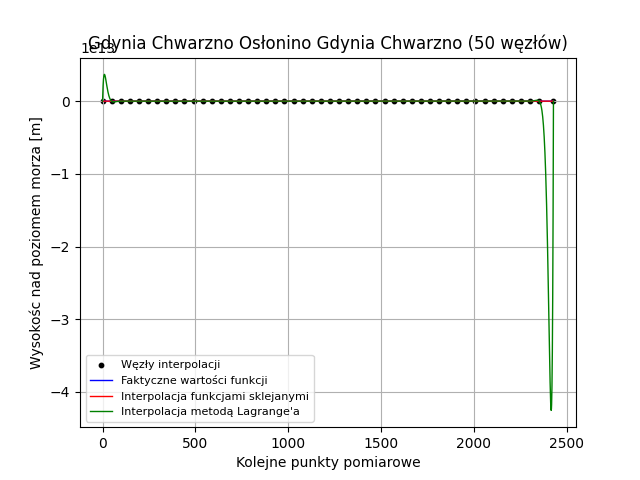
\includegraphics[width=\linewidth]{efektRungego.png}
          \caption{Przykład dla n = 50}
          \label{fig:sub2}
        \end{subfigure}
        \caption{Efekt Rungego}
        \label{fig:test}
    \end{figure}

    \noindent Jak widać na powyższych wykresach, metoda Lagrange'a dla dużych n daje bardzo złe rezultaty, a dla mniejszych n, dokładność interpolacji może nie być zadowoalająca.
    Sprawia to, że metoda ta jest średnio przydatna, szczególnie jeżeli zależy nam na sotsunkowo dokładnym wyznaczeniu funkcji interpolującej.

\newpage
\section{Interpolacja funkcjami sklejanymi}
    W metodzie interpolacji funckjami sklejanymi stosujemy interpolacje lokalną - dla każdego przedziału stosujemy interpolacje wielomianem niskiego stopnia.
    Pozwala to na uzyskanie dobrej dokładności przy jednoczesnym braku efektu Rungego.

    \noindent To rozwiązanie jest jednak bardziej kosztowne obliczeniowo, ze względu na koniczeność ułożenia i rozwiązania ukłądu równań liniowych. 
    Ma to na celu wyznacznenie współczynników n wielomianów (po 1 na przedział interpolacji) 3 stopnia. Układ ten będzie zatem zawierał 4n równań i 4n niewiadomych

    \noindent Konstrukcja układu:
    \begin{itemize}
        \item $S_i(x_i) = f(x_i)$ - ustalona wartość w węzłach interpolacji
        \item $S_i(x_{i+1}) = f(x_{i+1})$ - ciągłość funckji w węzłach
        \item $S_i'(x_{i+1}) = S_{i+1}'(x_{i+1})$ - ciągłość pierwszej pochodnej w węzłach
        \item $S_i''(x_{i+1}) = S_{i+1}''(x_{i+1})$ - ciągłość drugiej pochodnej w węzłach
        \item $S_0''(x_0) = 0, \; S_{n-1}''(x_n) = 0 $ - zerowanie drugiej pochodnej w węzłach granicznych
    \end{itemize}
\end{document}